
\begin{frame}
  \frametitle{Prediction Using Processed Gamma Spectra}
  \begin{figure}
    \centering
    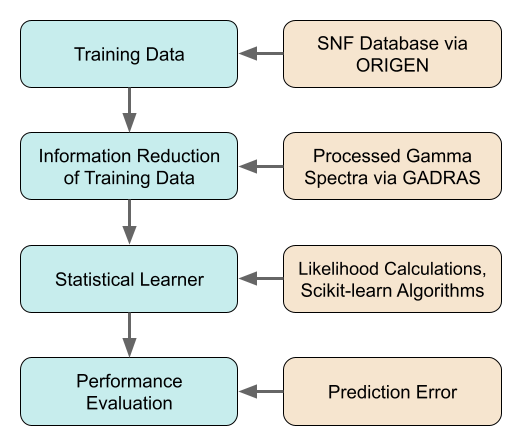
\includegraphics[width=0.6\textwidth]{./figures/methodology2.png}
  \end{figure}
\end{frame}

\begin{frame}
  \frametitle{Information Reduction: Processed Gamma Spectra}
  \begin{enumerate}
    \item Computational gamma detection \cite{gadras} 
    \item Process spectra: choose energy windows / window size
    \item Apply statistical counting error ($\sqrt{n}$) (using methods on previous slide)
  \end{enumerate}
  \begin{table}
    \small
    \centering
    \begin{tabular}{@{}lcllll@{}}
    \toprule
      \textbf{Detector} &
      \textbf{\begin{tabular}[c]{@{}c@{}}\% FWHM \\ @ 661 keV\end{tabular}} &
      \textbf{\begin{tabular}[c]{@{}l@{}}Distance \\ (cm)\end{tabular}} &
      \textbf{\begin{tabular}[c]{@{}l@{}}Height \\ (cm)\end{tabular}} &
      \textbf{\begin{tabular}[c]{@{}l@{}}Live Time\\ (s)\end{tabular}} &
      \textbf{\begin{tabular}[c]{@{}l@{}}Num \\ Channels\end{tabular}} \\ \midrule
      In-Lab HPGe           & 0.21 & 100.0 & 84.0  & 600  & 8192 \\
      Portable HPGe         & 0.29 & 100.0 & 100.0 & 600  & 8192 \\
      CZT                   & 1.20 & 100.0 & 100.0 & 600  & 1024 \\
      SrI\textsubscript{2}  & 2.94 & 100.0 & 100.0 & 600  & 1024 \\
      LaBr\textsubscript{3} & 3.63 & 213.0 & 84.5  & 2400 & 1024 \\
      NaI                   & 7.74 & 213.0 & 85.4  & 2400 & 1024 \\ \bottomrule
    \end{tabular}
  \end{table}
\end{frame}

\begin{frame}
  \frametitle{Gamma Spectra Processing}
  \begin{figure}
    \centering
    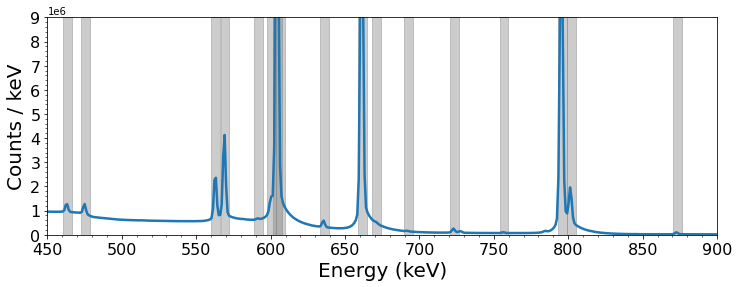
\includegraphics[width=\textwidth]{./figures/energy_window_example.png}
  \end{figure}
\end{frame}

\begin{frame}
  \frametitle{Gamma Spectra Processing}
  \begin{table}
    \small
    \centering
    \begin{tabular}{@{}lcm{0.5in}m{0.5in}m{0.5in}@{}}
      \toprule
      \multirow{2}{*}{\textbf{Detector}} &
      \multirow{2}{*}{\textbf{\begin{tabular}[c]{@{}l@{}}Energy Window\\ Size {[keV]}\end{tabular}}} &
      \multicolumn{3}{c}{\textbf{\# of Energy Windows}} \\ \cmidrule(l){3-5}
                       &    & Auto & Short & Long \\
      \toprule
      In-Lab HPGe      & 2  & 206  & 42    & 151  \\
      Portable HPGe    & 3  & 120  & 42    & 151  \\
      CZT              & 8  & 30   & 42    & 151  \\
      $\text{SrI}_2$   & 10 & 17   & 42    & 151  \\
      $\text{LaBr}_3$  & 12 & 19   & 42    & 151  \\
      NaI              & 12 & 9    & 42    & 151  \\ 
      \bottomrule
    \end{tabular}
  \end{table}
  \begin{table}
    \centering
    \renewcommand{\arraystretch}{1.3}
    \begin{tabular}{@{}|l|l|l|@{}}
      \hline
      \allbold{${}^{241}\text{Am}$} & \allbold{${}^{243}\text{Am}$} & ${}^{243}\text{Cm}$           \\ \hline
      ${}^{244}\text{Cm}$           & ${}^{245}\text{Cm}$           & \allbold{${}^{134}\text{Cs}$} \\ \hline
      \allbold{${}^{137}\text{Cs}$} & ${}^{152}\text{Eu}$           & \allbold{${}^{154}\text{Eu}$} \\ \hline
      \allbold{${}^{85}\text{Kr}$}  & ${}^{238}\text{Pu}$           & \allbold{${}^{125}\text{Sb}$} \\ \hline
    \end{tabular}
  \end{table}
\end{frame}

\begin{frame}
  \frametitle{Predictions with Decreasing Detector Energy Resolution}
  \begin{figure}
    \centering
    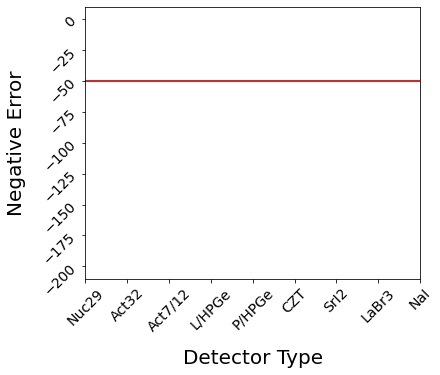
\includegraphics[height=0.7\textheight]{./figures/plot_description.png}
  \end{figure}
\end{frame}

\begin{frame}
  \frametitle{Reactor Type Classification}
  \begin{adjustwidth}{-15pt}{-10pt}
  \begin{figure}
    \centering
    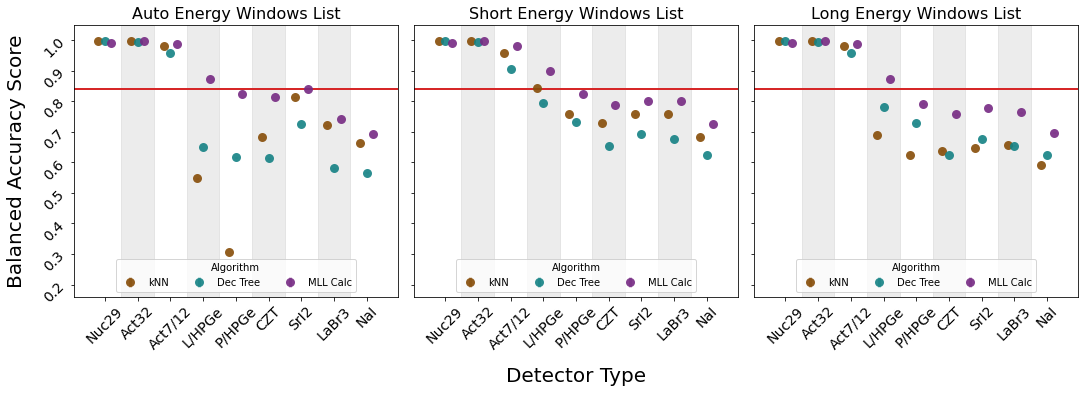
\includegraphics[width=1.1\textwidth]{./figures/detector_preds_wrt_enlist_BalAcc_rxtr.png}
  \end{figure}
  \vspace{12pt} \centering Red baseline: 0.84 balanced accuracy score
  \end{adjustwidth}
\end{frame}

\begin{frame}
  \frametitle{Reactor Type Classification}
  \begin{minipage}{0.5\textwidth}
    \begin{figure}
      \centering
      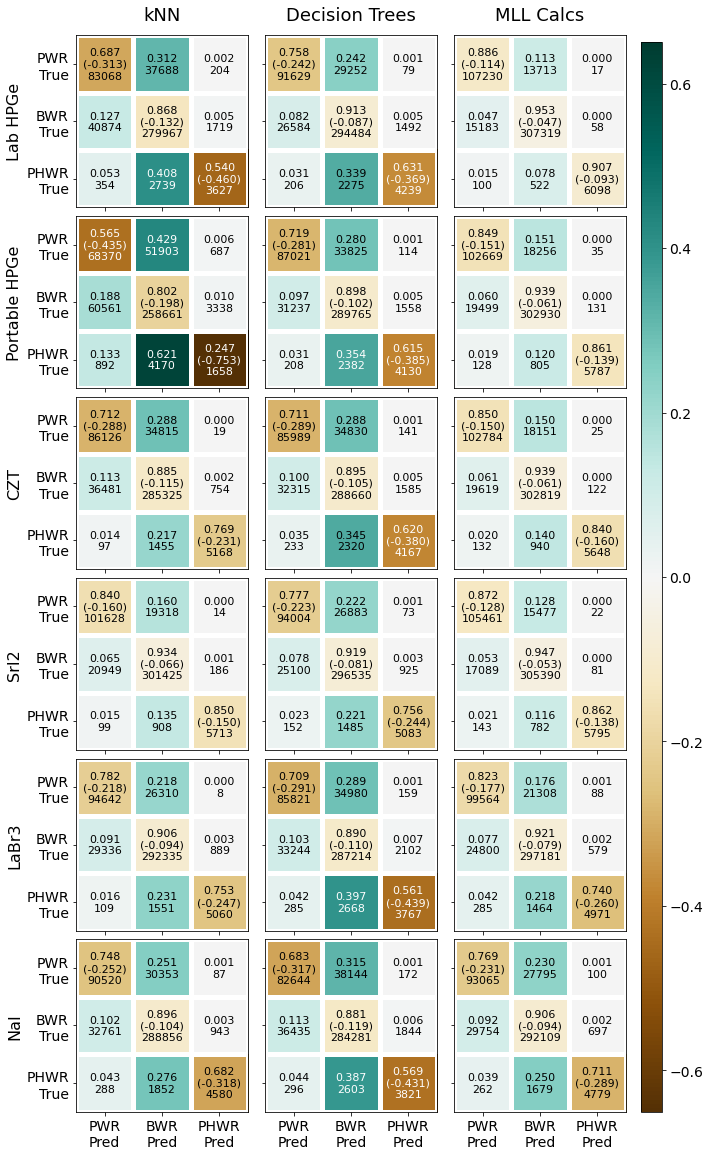
\includegraphics[height=0.88\textheight]{./figures/confusion_matrix_6dets_auto.png}
    \end{figure}
  \end{minipage}%
  \begin{minipage}{0.5\textwidth}
    \begin{figure}
      \centering
      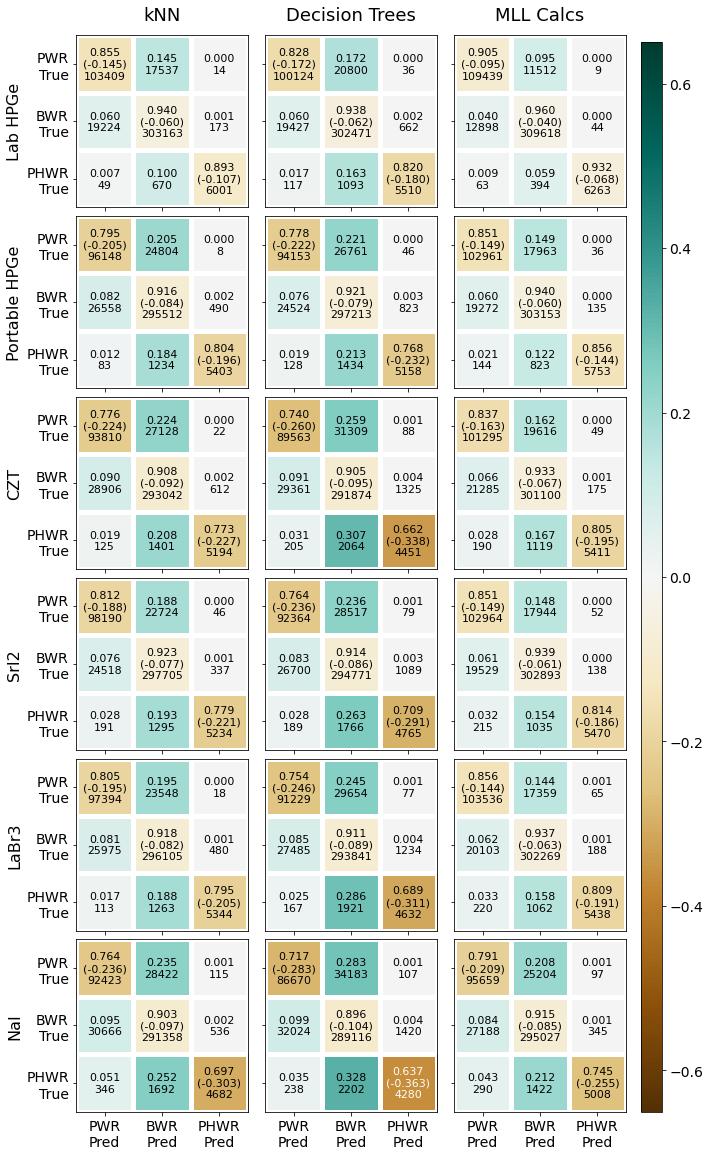
\includegraphics[height=0.88\textheight]{./figures/confusion_matrix_6dets_short.png}
    \end{figure}
  \end{minipage}
\end{frame}

\begin{frame}
  \frametitle{Burnup Regression}
  \begin{adjustwidth}{-15pt}{-10pt}
  \begin{figure}
    \centering
    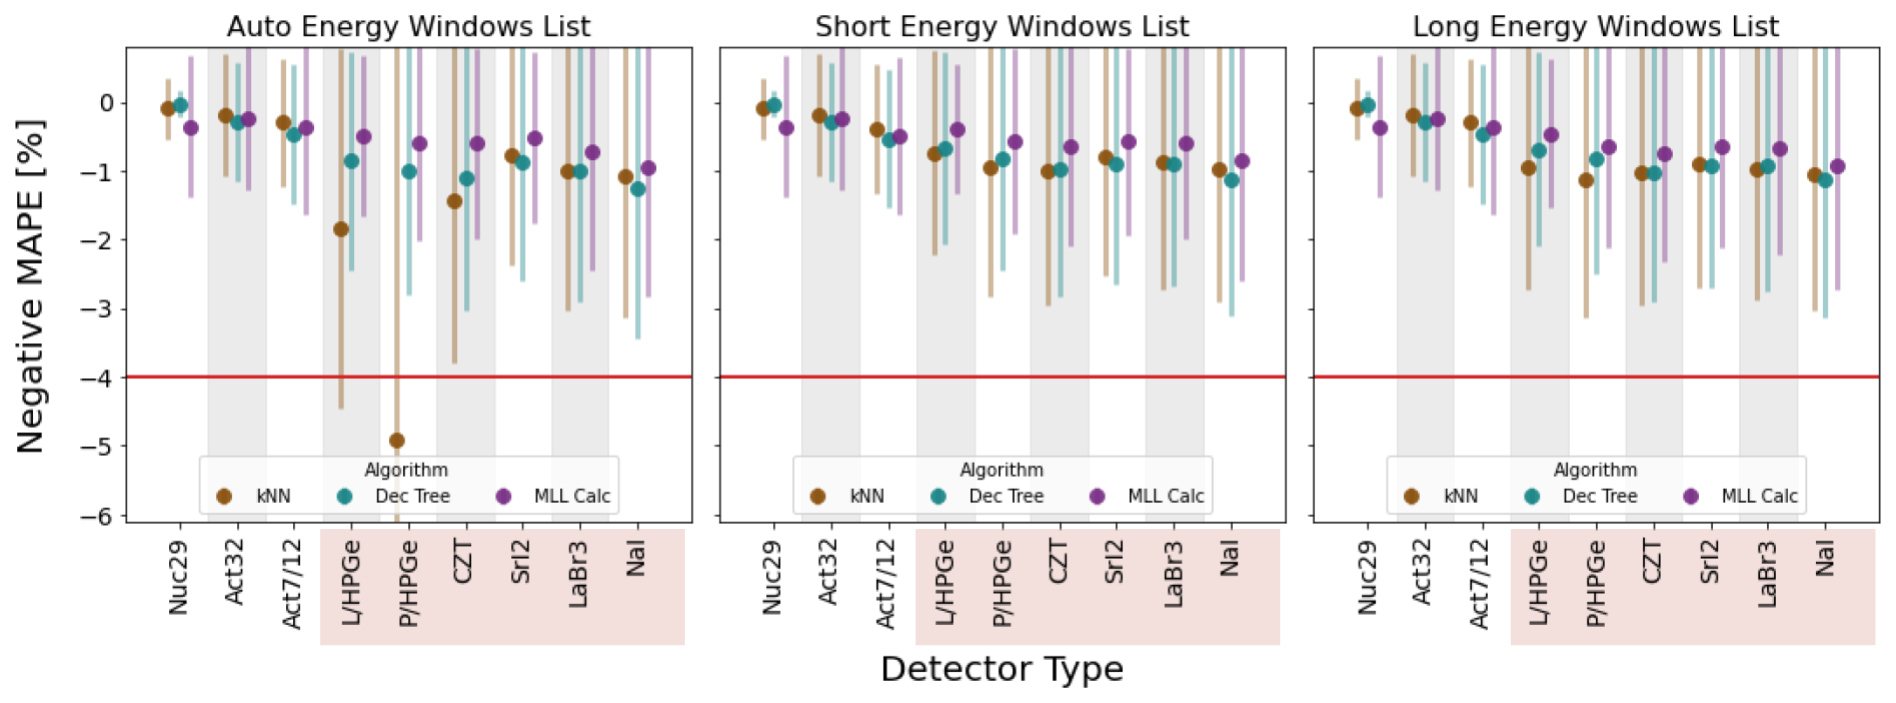
\includegraphics[width=1.1\textwidth]{./figures/detector_preds_wrt_enlist_MAPE_burn.png}
  \end{figure}
  \vspace{12pt} \centering Red baseline: -4\% 
  \end{adjustwidth}
\end{frame}

\begin{frame}
  \frametitle{Burnup Regression}
  \begin{adjustwidth}{-15pt}{-10pt}
  \begin{figure}
    \centering
    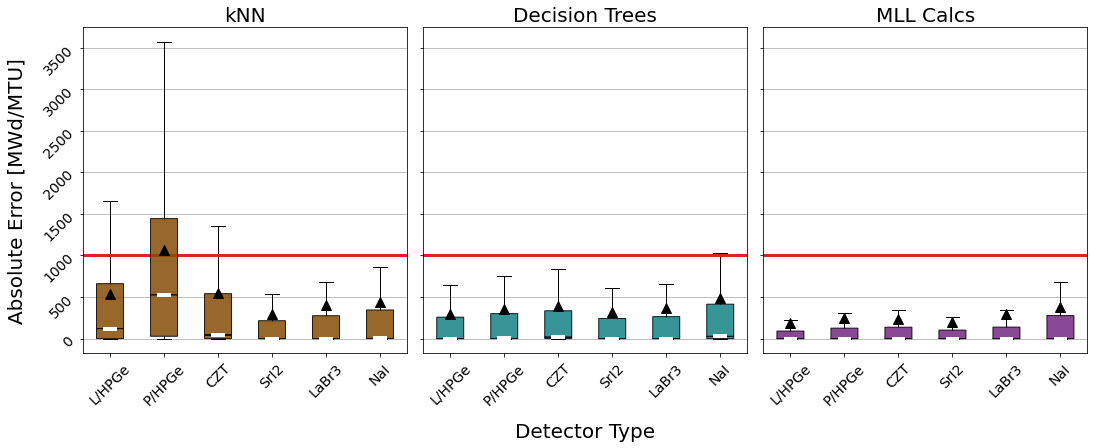
\includegraphics[width=1.1\textwidth]{./figures/abserror_boxplots_auto_burn.png}
  \end{figure}
  \vspace{12pt} \centering Red baseline: $1000\:MWd/MTU$; Outliers: $12-17\%$
  \end{adjustwidth}
\end{frame}

\begin{frame}
  \frametitle{Burnup Regression}
  \begin{adjustwidth}{-15pt}{-10pt}
  \begin{figure}
    \centering
    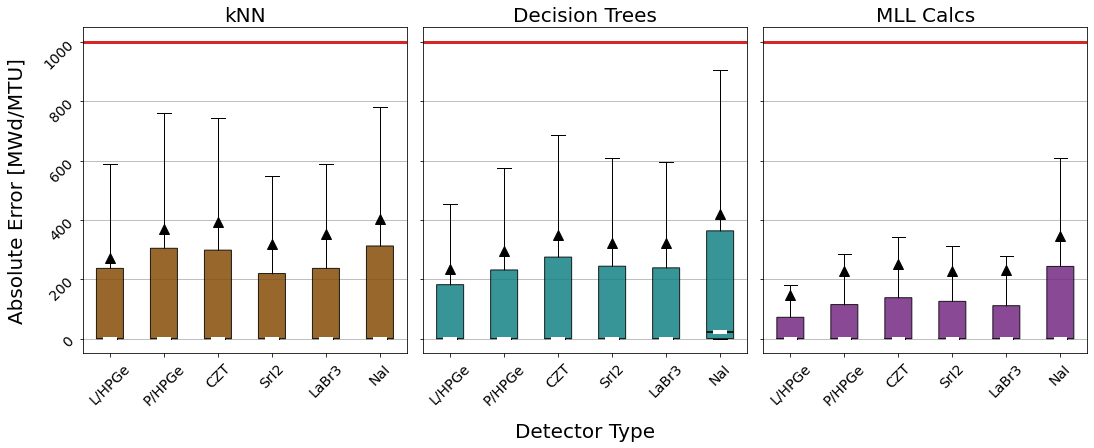
\includegraphics[width=1.1\textwidth]{./figures/abserror_boxplots_short_burn.png}
  \end{figure}
  \vspace{12pt} \centering Red baseline: $1000\:MWd/MTU$; Outliers: $12-17\%$
  \end{adjustwidth}
\end{frame}

\begin{frame}
  \frametitle{Burnup Regression}
  \begin{adjustwidth}{-15pt}{-10pt}
  \begin{figure}
    \centering
    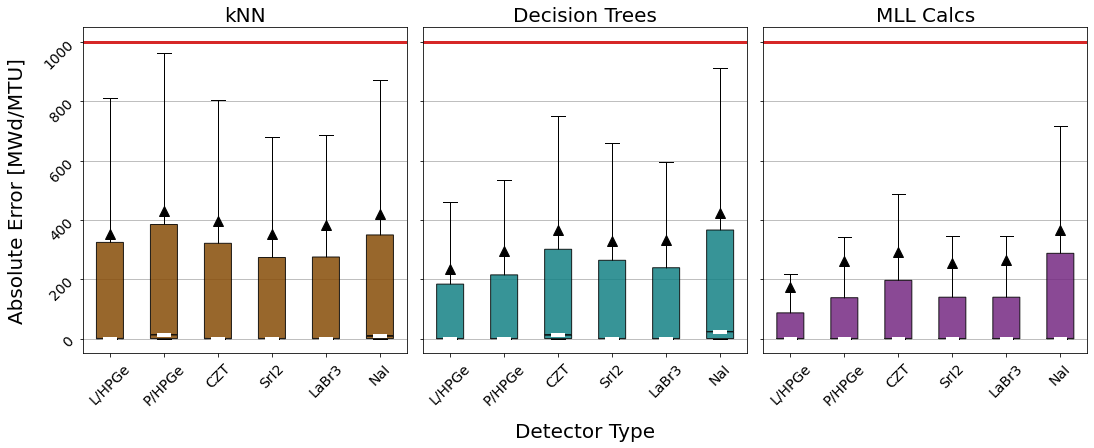
\includegraphics[width=1.1\textwidth]{./figures/abserror_boxplots_long_burn.png}
  \end{figure}
  \vspace{12pt} \centering Red baseline: $1000\:MWd/MTU$; Outliers: $12-17\%$
  \end{adjustwidth}
\end{frame}

\begin{frame}
  \frametitle{${}^{235}\text{U}$ Enrichment Regression}
  \begin{adjustwidth}{-15pt}{-10pt}
  \begin{figure}
    \centering
    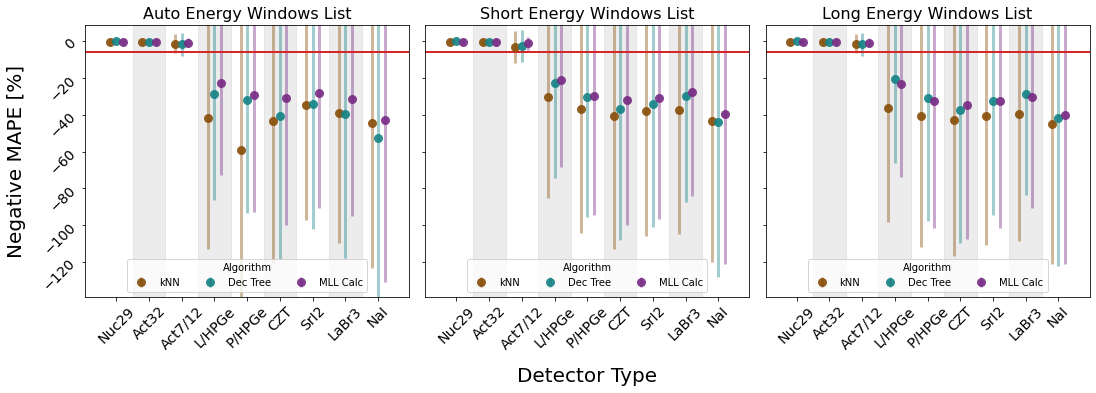
\includegraphics[width=1.1\textwidth]{./figures/detector_preds_wrt_enlist_MAPE_enri.png}
  \end{figure}
  \vspace{12pt} \centering Red baseline: -6\% 
  \end{adjustwidth}
\end{frame}

\begin{frame}
  \frametitle{${}^{235}\text{U}$ Enrichment Regression}
  \begin{adjustwidth}{-15pt}{-10pt}
  \begin{figure}
    \centering
    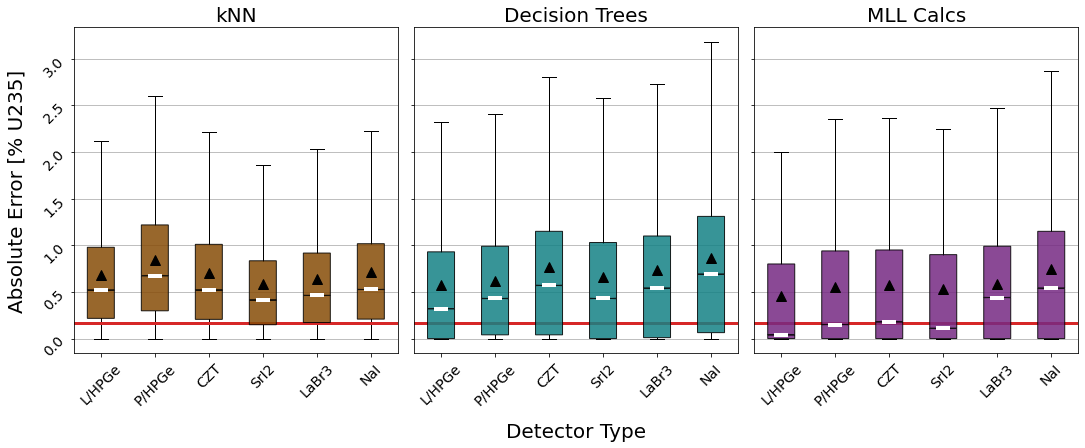
\includegraphics[width=1.1\textwidth]{./figures/abserror_boxplots_auto_enri.png}
  \end{figure}
  \vspace{12pt} \centering Red baseline: $0.17\%\:{}^{235}\text{U}$; Outliers: $3-4\%$
  \end{adjustwidth}
\end{frame}

\begin{frame}
  \frametitle{${}^{235}\text{U}$ Enrichment Regression}
  \begin{adjustwidth}{-15pt}{-10pt}
  \begin{figure}
    \centering
    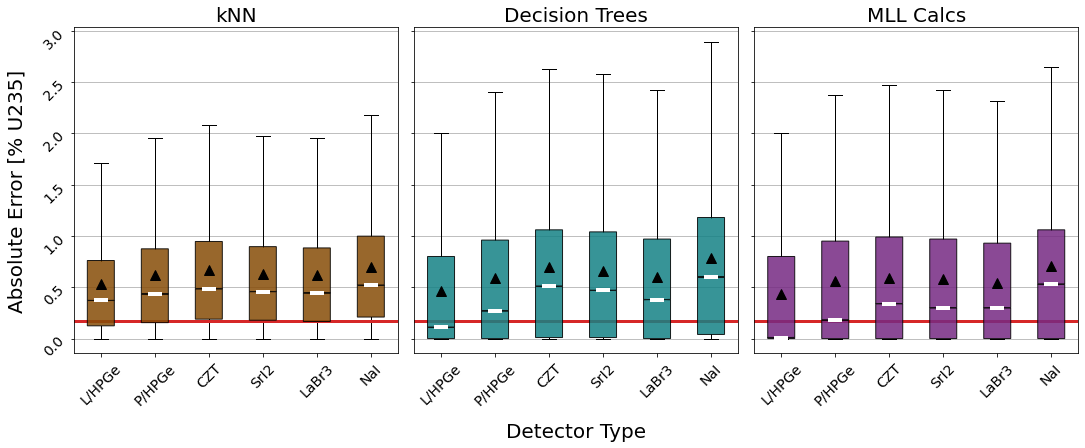
\includegraphics[width=1.1\textwidth]{./figures/abserror_boxplots_short_enri.png}
  \end{figure}
  \vspace{12pt} \centering Red baseline: $0.17\%\:{}^{235}\text{U}$; Outliers: $3-4\%$
  \end{adjustwidth}
\end{frame}

\begin{frame}
  \frametitle{${}^{235}\text{U}$ Enrichment Regression}
  \begin{adjustwidth}{-15pt}{-10pt}
  \begin{figure}
    \centering
    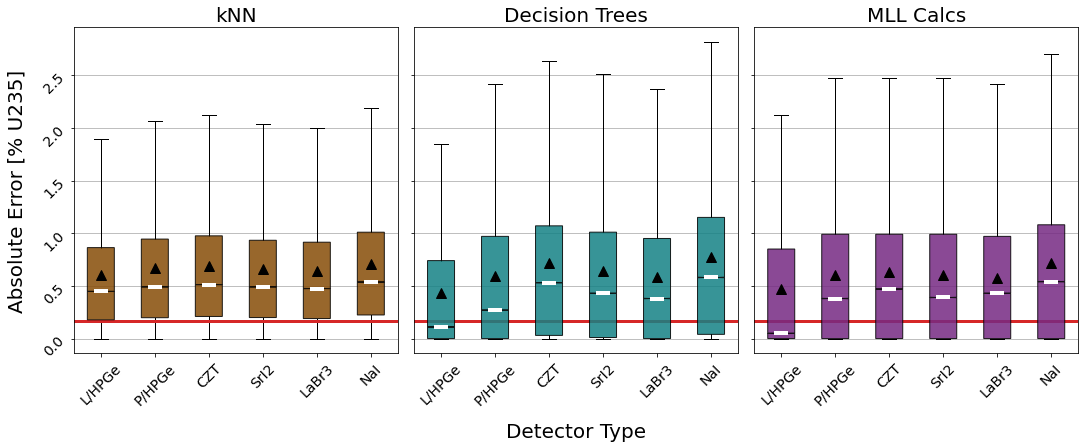
\includegraphics[width=1.1\textwidth]{./figures/abserror_boxplots_long_enri.png}
  \end{figure}
  \vspace{12pt} \centering Red baseline: $0.17\%\:{}^{235}\text{U}$; Outliers: $3-4\%$
  \end{adjustwidth}
\end{frame}

\begin{frame}
  \frametitle{Time Since Irradiation Regression}
  \begin{adjustwidth}{-15pt}{-10pt}
  \begin{figure}
    \centering
    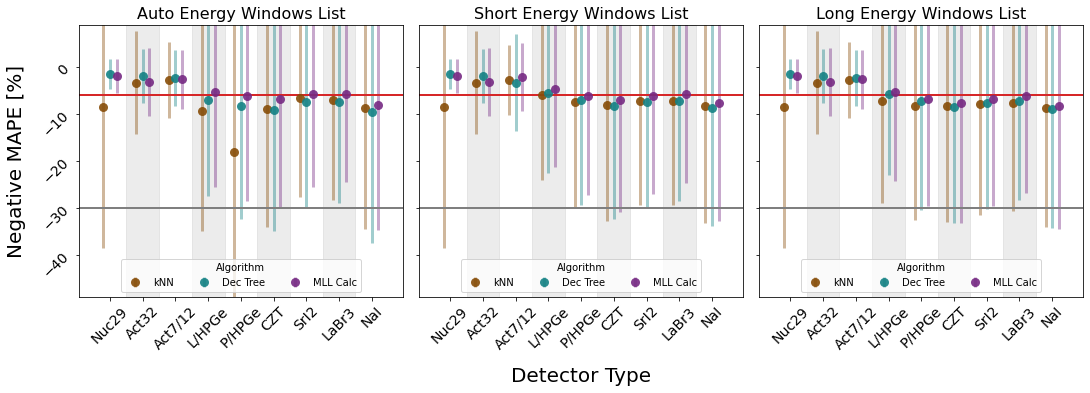
\includegraphics[width=1.1\textwidth]{./figures/detector_preds_wrt_enlist_MAPE_cool.png}
  \end{figure}
  \vspace{12pt} \centering Red baseline: -6\% (Grey line is -30\%) 
  \end{adjustwidth}
\end{frame}

\begin{frame}
  \frametitle{Time Since Irradiation Regression}
  \begin{adjustwidth}{-15pt}{-10pt}
  \begin{figure}
    \centering
    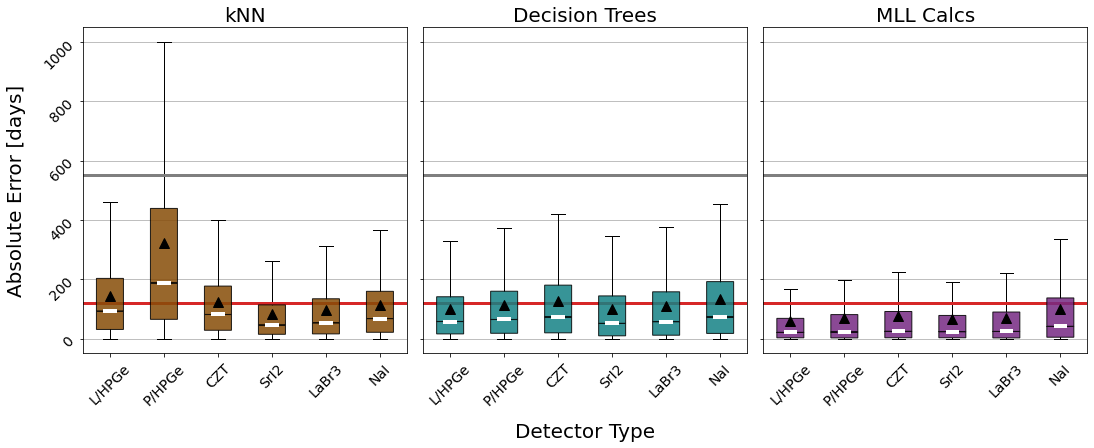
\includegraphics[width=1.1\textwidth]{./figures/abserror_boxplots_auto_cool.png}
  \end{figure}
  \vspace{12pt} \centering Red baseline: $120\:days$ (Grey line is $550\:days$); Outliers: $6-9\%$ 
  \end{adjustwidth}
\end{frame}

\begin{frame}
  \frametitle{Time Since Irradiation Regression}
  \begin{adjustwidth}{-15pt}{-10pt}
  \begin{figure}
    \centering
    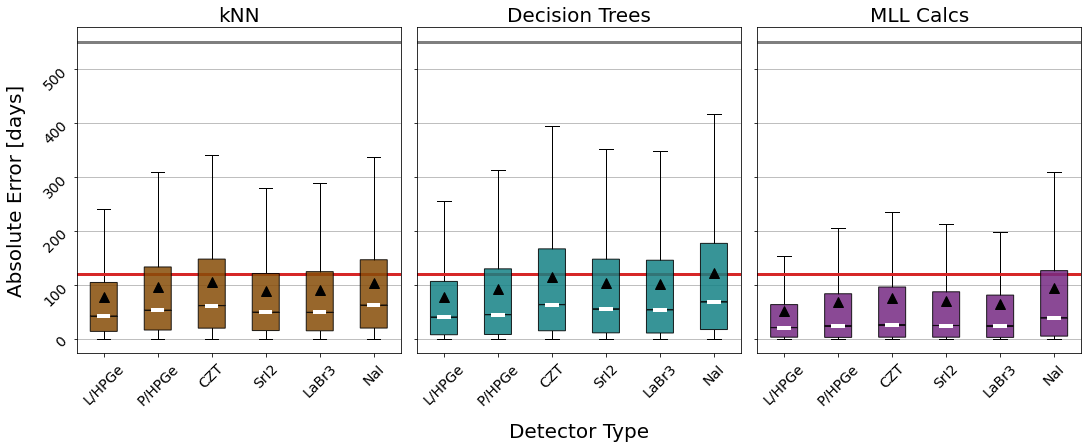
\includegraphics[width=1.1\textwidth]{./figures/abserror_boxplots_short_cool.png}
  \end{figure}
  \vspace{12pt} \centering Red baseline: $120\:days$ (Grey line is $550\:days$); Outliers: $6-9\%$  
  \end{adjustwidth}
\end{frame}

\begin{frame}
  \frametitle{Time Since Irradiation Regression}
  \begin{adjustwidth}{-15pt}{-10pt}
  \begin{figure}
    \centering
    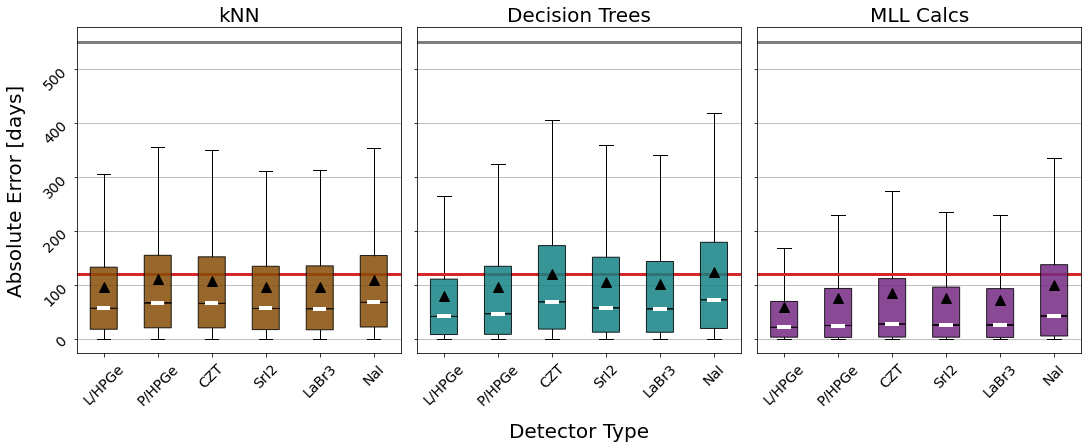
\includegraphics[width=1.1\textwidth]{./figures/abserror_boxplots_long_cool.png}
  \end{figure}
  \vspace{12pt} \centering Red baseline: $120\:days$ (Grey line is $550\:days$); Outliers: $6-9\%$  
  \end{adjustwidth}
\end{frame}

\begin{frame}
  \frametitle{Experiment Summary}
  \begin{itemize}
    \item Reactor type classification only exceeds threshold for four detector
    cases
    \item Burnup regression well exceeds the standard
    \item ${}^{235}\text{U}$ enrichment regression performs well below the
    standard
    \item Time since irradiation regression performs on or near the baseline
    \item Results are for the most part independent of gamma spectra processing 
    approach
  \end{itemize}
\end{frame}

